\documentclass[7pt]{article}
\usepackage[left=1in, right=1in, top=1in, bottom=1in]{geometry}
\usepackage[latin1]{inputenc}
\usepackage{amsmath}
\usepackage{amsfonts}
\usepackage{amssymb}
\usepackage{graphicx}
\author{Ben Larson}
\title{Homework 5 }
\date{Octt 5, 2016} 
\begin{document}
	\maketitle
	\section{6.4 Sherman-Morrison formula}
	We want to show that eqn 6.24 is the inverse of 6.25.\\
	Starting with the secant equations we can speculate that $B^{-1}$ is related to $ H$. 
	$$ H_{k+1}y_k=s_k $$
	$$ y_k = B_{k+1}s_k$$The sherman-morrison formula stats that when doing a rank update to a matrix the inverse of the new matrix is related to the old inverted matrix with some modification.
	$$\hat{A} = A+UV^T $$
	$$ \hat{A}^{-1} = A^{-1}-A^{-1}U(I+V^TA^{-1}U)^{-1}V^TA^{-1} $$
	 This is great as it allows you to find the inverse without having to actually solve for the inverse.  To show that $H_{k+1} $ is the inverse of$ B^{-1}_{k+1}$ we first plug in A, U, and V. 
	 $$ H_{k+1} = H_k -H_kU(I_k+V^TH_kU)^{-1}V^TH_K$$
	 We say that U and V are the same vector $v=y_k-B_ks_k$ that was used to derive the SR1 update. 
	 $$ H_{k+1} = H_k -H_k(y_k-B_ks_k)(I_k+(y_k-B_ks_k)^TH_k(y_k-B_ks_k))^{-1}(y_k-B_ks_k)^TH_K$$
	 Assuming that $A^{-1}B = I$ we get: 
	 $$ H_{k+1}=H(k)+(s_k-H_ky_k)(I_k+(s_k-H_ky_k)^T(s_k-H_ky_k))^{-1}(s_k-H_ky_k)^T $$

	\section{Optimization for the Rosenbrock function}
	Note that I didn't get any of the functions to optimize correctly, therefore it would be meaningless to compare the results. There were a lot of parameters that I wasn't sure how to set that would give vastly different answers even with small changes in parameter settings. Most notably was the initial guess for $H_0 and \alpha_k$.
	$$ H_0 =\lambda I$$
	I tried many different $\lambda$ for SR1, BFGS and got very different results even with small changes in $\lambda$. I thought the algorithms would correct even bad guesses, but they did not. 
	\subsection{Conjugate Gradient}
	To solve the Rosenbrock function we need to use nonlinear conjugate gradient methods as the function is not a convex quadratic function. I used the Fletcher Reeves method. I used the algorithm as written out in the book. We iterate until the $\triangledown f = 0$. We find a step size for our directional derivative: $x_{k+1} = x_k + \alpha_k p_k$. The goal here is to find a good $\alpha$ and directional derivative $p_k$. Rather than using residuals: $r = Ax-b$ we use the gradient $\frac{\triangledown f_{k+1}^T\triangledown f_{k+1}}{\triangledown f_{k}^T\triangledown f_{k}}$. \\
	
	\subsection{BFGS}
	For BFGS we are using a optimization that avoids finding the Hessian of the function. We have to initially guess what the Hessian approximation $H_0$. I used the identity matrix. We compute a search direction $p_k=-H_k\triangledown f_k$. Then we do an update $x_{k+1} = x_k + \alpha_k p_k$. Then we use the secant equation. We are trying to avoid recomputing the Hessian matrix, so we use information about the previous iteration and update a reasonable value.
	$$H_{k+1} = (I-\rho_k s_k y_k^T)H_k(I-\rho_k s_k y_k^T)+\rho_k s_k y_k^T $$
	\subsection{SR1}
	This algorithm works by a rank 1 update: $B_{k+1} = B_k +\sigma VV^T$. Where v are usually new vectors that the algorithm is optimizing. Using the secant equation we end up with the formula: 
$$ B_{k+1} = B_k + \frac{(s_k - H_ky_k)(s_k - H_ky_k)^T}{(s_k - H_ky_k)^Ts_k} $$\\ 
For the steps in the algorithm we use the formula used in the book. A region trust method is employed that solves for the best vector within a trust region: $\delta_k$. Then based on this value the algorithm employs a series of logical steps to update  $x_k,\delta_k, B_k$. \\
\pagebreak
\begin{figure}
	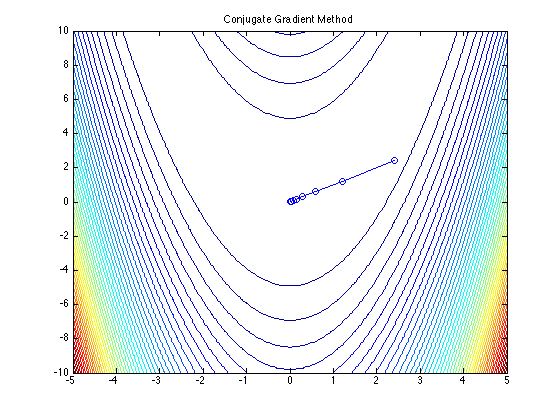
\includegraphics[width = 10cm]{conGrad}
	\caption{In this method $H_0= I+10^3$ with alpha set constant rather than using a line search. Possible problems with the algorithm is search direction. It should not be moving up the gradient.}
\end{figure}
\begin{figure}
	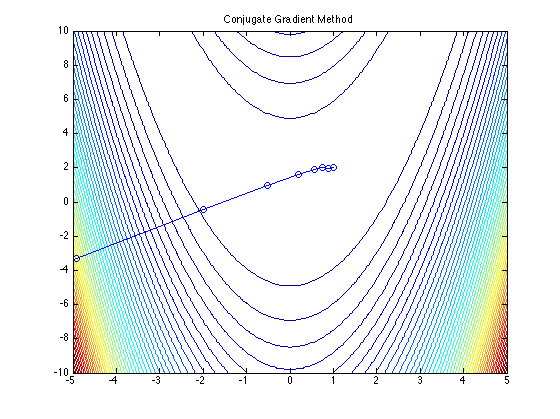
\includegraphics[width = 10cm]{conGrad12}\\
	\caption{In this conjugate gradient I used a line search to find the step size. Very wrong search direction. The search direction changed directions with initial $H_0=100, H_0=1000$. I saw both initial settings moving the up the gradient rather than down.}
\end{figure}
\begin{figure}
	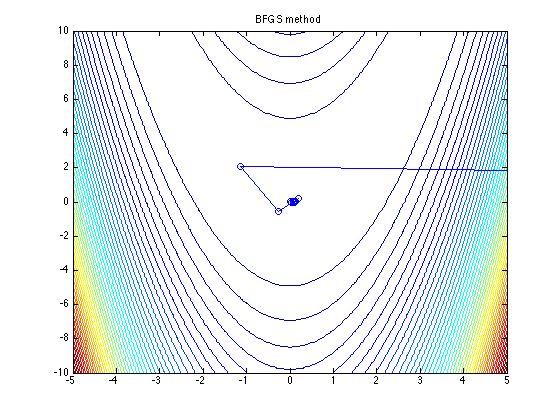
\includegraphics[width = 10cm]{bfgs0}\\
	\caption{BFGS looked promising for a few iterations, then fails miserably, making a huge jump into the gradient. This is due to an error somewhere in the search direction because the H seems to be well behaved.}
\end{figure}
\begin{figure}
	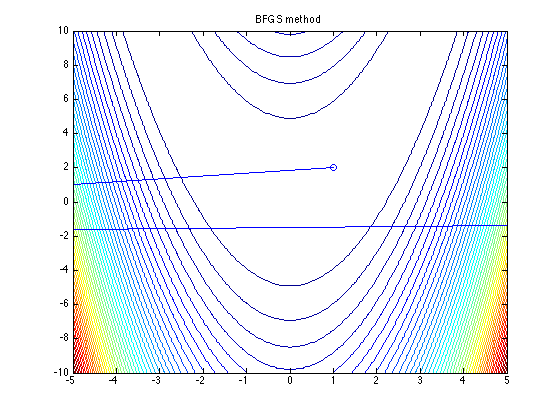
\includegraphics[width = 10cm]{bfgs21}\\
	\caption{BFGS this clearly shows a problem with the search direction. I haven't been able to find why this jump is happening. The algorithm uses $x_{k+1}= x_{k} + \alpha p$ to update x then even with forced small alpha the p jumps into enormous steps ruining any chance of optimal behavior. p is updated by H and gradient. }
\end{figure}
\begin{figure}
	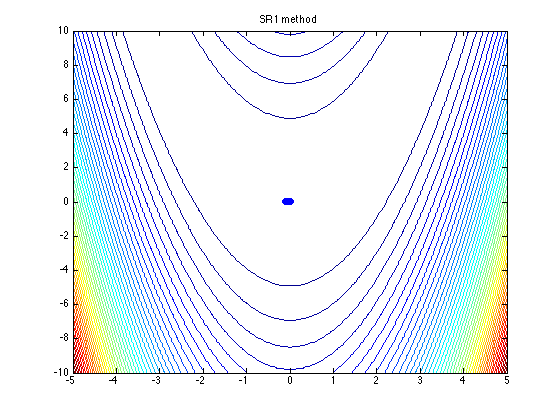
\includegraphics[width = 10cm]{sr1zero}\\
	\caption{This algorithm has so many parameters I'm not sure what to say is causing a failure.}
\end{figure}
\begin{figure}
	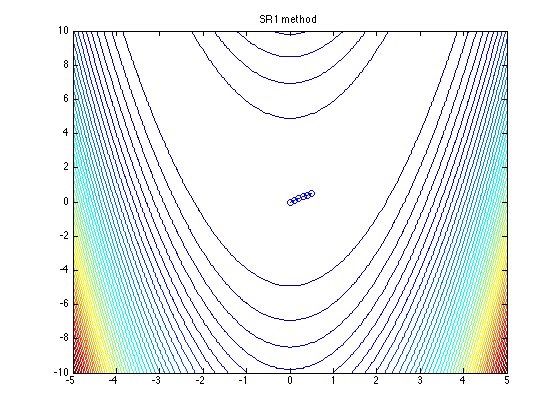
\includegraphics[width = 10cm]{sr10}\\
	\caption{With this starting point, maybe it is marching towards a minimum, but it should do so quickly as this uses a trust region, and the step size should be updated to become larger.}
\end{figure}
		\end{document} 